\section{Lineare Zeitinvariante System (LTI)}
\subsection{Laplace-Transformation}


 	\subsubsection{Eigenschaften}
  		\renewcommand{\arraystretch}{2}
		\begin{tabularx}{\textwidth}{|l|X|}
        	\hline
        	Linearität & 
 			$a\cdot f(t) + \beta\cdot g(t) \laplace a\cdot F(s) + \beta\cdot
 			G(s)$ \\
 			\hline
 			"Ahnlichkeit / Streckung &
 			$f(a t) \laplace \frac{1}{a}F \left (\frac{s}{a} \right ) \quad 0
 			<a \in\mathbb{R}$ \\
 			\hline
 			Faltung im Zeitbereich &
 			$f(t) \ast g(t) = \int\limits_{0}^{t} f(\tau)g(t-\tau)d\tau \laplace F(s)
 			\cdot G(s)$\\
 			\hline
 			Faltung im Frequenzbereich &
 			$f(t) \cdot g(t) \laplace \frac{1}{2\pi j}\int\limits_{c-j\infty}^{c+j\infty}
 			F(\xi) G(s-\xi)d\xi$ \\
 			\hline
 			Ableitung im Zeitbereich &
 			$\frac{\partial f(t)}{\partial t} \laplace sF(s)
 			-f(0^+)$ \\
 			\hline
 			Ableitungen im Zeitbereich &
 			$\frac{\partial^n f(t)}{\partial t^n} \laplace s^nF(s)
 			-s^{n-1}f(0^+)-s^{n-2}\frac{\partial f(0^+)}{\partial t}-\ldots
 			-s^0\frac{\partial^{n-1} f(0^+)}{\partial t^{n-1}}$ \\
 			\hline
 			Multiplikation mit $t$ &
 			$t\cdot f(t)  \laplace \frac{-\partial F(s)}{\partial s}$ \\
 			\hline
 			Ableitung im Frequenzbereich &
 			$(-t)^n f(t) \laplace  \frac{\partial^n F(s)}{\partial s^n}$ \\
 			\hline
 			Verschiebung im Zeitbereich nach rechts &
 			$f(t - t_0) \laplace F(s)e^{- t_0 s}$ \\
 			\hline
			Verschiebung im Zeitbereich nach links &
			$f(t + t_0) \laplace e^{t_0 s} \cdot [F(s) - \int\limits_0^{t_0} f(t) \cdot e^{-st} dt]$\\
			\hline
 			Verschiebung im Frequenzbereich (Dämpfungssatz) &
 			$f(t)e^{\mp a t} \laplace F(s\pm a)$ \\
 			\hline
 			Integration &
 			$\int\limits_0^t f(\tau)d\tau \laplace \frac{1}{s}F(s)$ \\
 			\hline
 			Anfangswerttheorem &
 			$\lim_{t\rightarrow 0^+} f(t) = \lim_{s\rightarrow \infty} s \cdot F(s),\text{~wenn
 			}  \lim_{t\rightarrow 0} f(t)\text{~existiert}.$ \\
 			\hline
 			Endwerttheorem &
 			$\lim_{t\rightarrow \infty} f(t) = \lim_{s\rightarrow 0} s \cdot F(s),\text{~wenn
 			}  \lim_{t\rightarrow \infty} f(t)\text{~existiert.}$ \\
 			\hline
       	\end{tabularx}
\newpage
	\subsubsection{Laplace-Tabelle}
	\begin{multicols}{2}
		\begin{center}
			\begin{tabular}{|lcc|}
				\hline
				$\delta \left( t \right)$ & $\laplace$ & $1$ \\
				$\delta \left( t - a \right)$ & $\laplace$ & $e^{- a s}$\\
				$\sigma \left( t \right)$ = $\varepsilon \left( t \right)$ & $\laplace$ & $\frac{1}{s}$ \\
				$\sigma \left( t \right) \cdot t$ & $\laplace$ & $\frac{1}{s^2}$\\
				$\sigma \left( t \right) \cdot t^2$ & $\laplace$ & $\frac{2}{s^3}$\\
				$\sigma \left( t \right) \cdot t^n$ & $\laplace$ & $\frac{n!}{s^{n+1}}$\\
				$\sigma \left( t \right) \cdot e^{a t}$ & $\laplace$ &
				$\frac{1}{s-a}$\\
				$\sigma \left( t \right) \cdot t \cdot e^{a t}$ & $\laplace$ &
				$\frac{1}{( s - a )^2}$\\
				$\sigma \left( t \right)\cdot t^2 \cdot e^{a t}$ &
				$\laplace$ & $\frac{2}{{( s - a )}^3}$\\
				$\sigma \left( t \right)\cdot t^n \cdot e^{ a t}$ &
				$\laplace$ & $\frac{n!}{(s-a)^{n+1}}$\\
				$\sigma \left( t \right) \cdot (1-e^{a t}$) & $\laplace$ &
				$\frac{- a}{s ( s - a )}$\\
				$\sigma \left( t \right) \cdot \cos \left(b t \right)$ & $\laplace$ &
				$\frac{s}{ s^2 + b^2}$\\
				$\sigma \left( t \right) \cdot \sin \left(b t \right)$ & $\laplace$ &
				$\frac{b}{s^2 + {b^2}}$\\
				$\sigma \left( t \right) \cdot e^{a t} \cdot \cos \left(b t \right)$ & $\laplace$ &
				$\frac{s- a}{ (s- a)^2 + b^2}$\\
				$\sigma \left( t \right) \cdot e^{a t} \cdot \sin \left(b t \right)$ & $\laplace$ &
				$\frac{b}{(s- a)^2 + {b^2}}$\\
				$\sigma \left( t \right) \cdot \frac{e^{a t} - e^{b t}}{a-b}$ & $\laplace$ & $\frac{1}{(s-a)(s-b)}$ \\
				$\sigma \left( t \right) \cdot \frac{a e^{a t} - b e^{b t}}{a-b}$ & $\laplace$ & $\frac{s}{(s-a)(s-b)}$\\
				\hline
			\end{tabular}
		\end{center}
	\columnbreak
		\begin{center}
	\[\boxed{F(s)=\int\limits_0^\infty f(t)e^{-st}dt} \qquad s=\sigma+j\omega\]\\
\subsubsection{Bedingungen}
\begin{itemize}
		\item Definitionsbereich nur für kausale Systeme $t\geq 0$\\
		\item Integrierbar über das Intervall $(0,\infty)$\\
		\item Wachstum kleiner als der von eienr Exponentialfunktion\\ 
		\item Gegen"uber $j\omega$ bei der Fourier-Transformation ist bei der
			Laplace-Transformation $s$ verallgemeinert zu $s=\sigma + j\omega$. Das
			bedeutet, dass die Fourier-Transformierte $F(j\omega)$ durch die
			Laplace-Transformation $F(s)$ ausgedr\"uckt werden kann. \\
		\item mit $\sigma = 0 \rightarrow$ Amplitude bleibt konstant\\
		\item mit $\sigma > 0 \rightarrow$ explodiert die Amplitude f\"ur $0 < t \rightarrow \infty$ \\
		\item mit $\sigma < 0 \rightarrow$ klingt die Amplidute für $0 < t \rightarrow \infty$ auf $0$ ab
\end{itemize}

	\subsubsection{Vorgehen Rücktransformation}
		\begin{enumerate}
			\item Kürzen oder vereinfachen
			\item Rücktransformation mittels Laplace-Tabelle
			\item Partialbruchzerlegung falls nötig
			\item $h(t)\hspace{0.2cm}\underline{nicht} < 0$
		\end{enumerate}
	\end{center}
\end{multicols}

\subsection{Differentialgleichungen lösen}
Die ‘interne’ Beschreibung transformieren, fallen Probleme mit Anfangsbedingungen weg, da man näher
an den physikalischen Grössen bleibt
\begin{multicols}{2}
		\begin{center}
			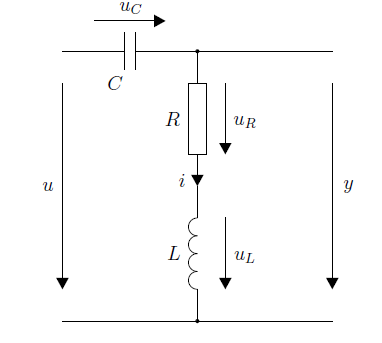
\includegraphics[width=6cm]{./images/diffgleichung.png}
		\end{center}
	\columnbreak
\begin{center}
	\begin{tabular}{ll}
		$i(t) = C \cdot \dot{u}_{C}(t)$ & Kapazität  \\
		$u_{L}(t) = L \cdot \dot{i}(t)$ & Induktivität \\
		$u_{R}(t) = R \cdot i(t)$ & Widerstand \\
		$u(t) = u_{C}(t) + u_{R}(t) + u_{L}(t)$ & Maschengleichung, links \\
		$y(t) = u_{R}(t) + u_{L}(t)$ & Maschengleichung, rechts \\
	\end{tabular}
\end{center}
\end{multicols}

\begin{multicols}{2}
{	$I(s) = C  \cdot  [s  \cdot  U_{C}(s) - u_{C}(0)]$ \\
	$U_{L}(s) = L  \cdot  [s  \cdot  I(s) - i(0)]$ \\
	$U_{R}(s) = R  \cdot  I(s)$ \\
	$U(s) = U_{C}(s) + U_{R}(s) + U_{L}(s)$ \\
	$Y (s) = U_{R}(s) + U_{L}(s)$ \\}

	\columnbreak
\begin{center}

$Y(s) = \frac{s^2 LC+sRC}{s^2 LC +sRC +1}\cdot U(s) + \frac{[sLC + RC] \cdot u_{C}(0) + L \cdot i(0)}{s^2 LC +sRC +1}$
\end{center}
\end{multicols}

Auch hier beinhaltet das Gleichungssystem 5 Gleichungen und 6 Signale. Das Eliminieren der 4 internen Signale $(U_{C}, U_{R}, U_{L}, I)$ fällt hier leichter. Offensichtlich sind hier weniger Anfangsbedingungen nötig als wenn nur eine Gleichung in den Bildbereich transformiert wird.


\subsection{Partialbruchzerlegung (PBZ)}
\subsubsection{Allgemeines Vorgehen}			\[f(x)=\frac{x^2+20x+149}{x^3+4x^2-11x-30} \Rightarrow \; \Rightarrow x^{3}+4x^{2}-11x-30=(x+2)(x^{2}+2x-15)=(8x+2)(x+5)(x-3)\]
			Ansatz:
			\[f(x)=\frac{x^2+20x+149}{x^3+4x^2-11x-30}=\frac{A}{x-3} + \frac{B}{x+2} + \frac{C}{x+5}=
			\frac{A(x+2)(x+5)+B(x-3)(x+5)+C(x-3)(x+2)}{(x-3)(x+2)(x+5)}\]
			Gleichungssystem \textbf{(Z"ahler gleichsetzen)} aufstellen mit beliebigen $x_i$-Werten (am Besten Polstellen oder 0,1,-1 w"ahlen):
			\[\begin{array}{l}x_1=3:\;-9+60+149=A\cdot5\cdot8\;\;\;\Rightarrow A=5\\
			x_2=-2:\;-4-40+149=B(-5)\cdot3\; \Rightarrow B=-7\\
			x_3=-5:\;-25-100+149=C(-8)(-3) \Rightarrow C=1 \end{array} \Rightarrow f(x)=\frac{5}{x-3}+\frac{7}{x+2} + \frac{1}{x+5}\]
%			weitere Ans"atze f"ur andere Typen von Termen: (Mehrere Werte f"ur $x$ verwenden, auch wenn kein Koeffizient 0 wird.)
%			\[f(x)=\frac{5x^2-37x+54}{x^3-6x^2+9x}=\frac{A}{x}+\frac{B}{x-3}+\frac{C}{(x-3)^2}=\frac{A(x-3)^2+Bx(x-3)+Cx}{x(x-3)^2}\]
%			\[f(x)=\frac{1,5x}{x^3-6x^2+12x-8}=\frac{A}{x-2}+\frac{B}{(x-2)^2}+\frac{C}{(x-2)^3}=\frac{A(x-2)^2+B(x-2)+C}{(x-2)^3}\]
%			\[f(x)=\frac{x^2-1}{x^3+2x^2-2x-12}=\frac{A}{x-2}+\frac{Bx+C}{x^2+4x+6}=\frac{A(x^2+4x+6)+(Bx+C)(x-2)}{(x-2)(x^2+4x+6)}\]
\subsubsection{Bedingungen}
\begin{itemize}
\item Bedingung 1: In der gezeigten Form kann die PBZ nur durchgeführt werden,
wenn die Pole paarweise verschieden sind: $p_{i} \neq p_{j}$ falls i $\neq$ j.
\item Bedingung 2: In der gezeigten Form kann die PBZ nur durchgeführt werden, wenn m < n. Die Schrittantwort des Systems ist dann stetig.
\item Bei komplex-konjugierten Polen $p_{j} = p^{\ast}_{i}$ ergeben sich komplex-konjugierte Faktoren
$c_{j} = c^{\ast}_{i}$ . Werden die entsprechenden zwei Terme addiert, ergeben sich
für die Summe reelle Koeffizienten (PT2-Glied):
\end{itemize}
\subsubsection{Standardfall}

\[ G(s) =\frac{c_{1}}{s+3} + \frac{c_{2}}{s+5} + \frac{c_{3}}{s+7} \quad \text{ mit } \quad {c_{i}= \frac{Z(s)}{\frac{dN(s)}{ds}}\mathop{\Bigg|}\limits_{s=p_{i}}}\]

Beispiel: \[\frac{22s +35}{(s+1)(s+2)}=\frac{c_{1}}{s+1}+\frac{c_{2}}{s+2}=\frac{\frac{22s+35}{2s+3}\mathop{\Big|}\limits_{s=-1}}{s+1}+\frac{\frac{22s+35}{2s+3}\mathop{\Big|}\limits_{s=-2}}{s+2}=\frac{13}{s+1}+\frac{9}{s+2}\]
kann durch PBZ in drei parallel geschaltete PT1-Glieder umgeformt werden. Die
Faktorisierung ist dabei nur beim Nenner nötig.

\subsubsection{Nichtminimale Übertragungsfunktion}
\[G(s) =\frac{8s^{2} + 80s + 200}{s^3 + 15s^2 + 71s + 105}= \frac{4}{s+3} + \frac{0}{s+5} + \frac{4}{s+7}\]
Die in (27) gegebene UTF scheint zwar ein System dritter Ordnung zu sein; die beiden
folgenden Darstellungen zeigen aber, dass das I/O-Verhalten nur einem System
zweiter Ordnung entspricht. In der faktorisierten Form äussert sich dies durch
eine Pol-/Nullstellenkürzung; in der PBZ ist der entsprechende Koeffizient $c_{2}$ = 0.
Die UTF in ist nicht minimal; eine vollständig gekürzte UTF dagegen heisst
minimal.

\subsubsection{Übertragungsfunktion mit komplexen Polen}
\[G(s) =\frac{8s^{2} + 70s + 134}{s^3 + 15s^2 + 81s + 175}= \frac{8s^2+70s+134}{(s+7)(s+4+3j)(s+4-3j)}=\frac{2}{s+7}+\underbrace{\frac{3+2j}{s+4-3j}+\frac{3-2j}{s+4+3j}}\]
\textcolor{white}{x} \hspace{14.5cm} $\frac{6s+12}{s'2+8s+25}$\\

Grundsätzlich kann G(s) wieder als Parallelschaltung dreier PT1-Glieder aufgefasst
werden. Glieder mit komplexen Werte für Verstärkung und Zeitkonstante werden
üblicherweise aber zu Teilsystemen zweiter Ordnung zusammengefasst.

\subsubsection{Fall m $>$ n}
UTF mit m $>$ n haben bei hohen Frequenzen differentierendes Verhalten, mit m = n
haben sie bei hohen Frequenzen Proportionalverhalten. Um solche UTF in eine
parallele Form zu bringen, kann mit einer Polynomdivision gearbeitet werden. Die Polynomdivision wird abgebrochen, bevor negative s-Potenzen entstehen. Terme mit nicht-negativen s-Potenzen haben proportionales
bzw. differentierendes Übertragungsverhalten; bei höheren s-Potenzen träte auch
mehrfache Differentiation auf. Wenn ein übrig bleibt, so kann dieser mit PBZ weiter zerlegt werden.

\subsection{Darstellung und Eigenschaften von UTF}

\begin{eqnarray}
G(s)=\frac{Z(s)}{N(s)}=\frac{b_{m}s^m + b_{m-1}s^{m-1}+ ... + b_{1}s+b_{0}}{s^{n}+a_{n-1}s^{n-1} + ... + a_{2}s^{2}+a_{1}s + a_{0}} \\ = K\cdot \frac{(s-z_{1})(s-z_{2})...(s-z_{m})}{(s-p_{1})(s-p_{2})...(s-p_{n})} \\ = \frac{c_{1}}{s-p_{1}} + \frac{c_{2}}{s-p_{2}} + ...  + \frac{c_{n}}{s-p_{n}}
\end{eqnarray}

\begin{equation}
K=b_{m}
\end{equation}
\subsubsection{Übertragungsfunktion UTF}
\hspace{2.3cm}G(s)\\
$Y(s) = \underbrace{\frac{\overbrace{s^2 LC+sRC}}{s^2 LC +sRC +1}\cdot U(s)} + \underbrace{\frac{[sLC + RC] \cdot u_{C}(0) + L \cdot i(0)}{s^2 LC +sRC +1}}$ \newline
\textcolor{white}{x} \hspace{2.4cm} $Y_{E}(s)$ \hspace{3.8cm} $Y_{F}(s)$ \\
Das Ausgangssignal Y (s) setzt sich aus den beiden Termen $Y_{E}(s) und Y_{F}(s)$ zusammen.Der erzwungene Anteil $Y_{E}(s)$ ist durch das Eingangssignal U(s) bestimmt, aber unabhängig von den Anfangsbedingungen des Netzwerks.
Beim freien Anteil $Y_{F}(s)$ ist es umgekehrt; dieser hängt nur von den Anfangsbedingungen,
nicht aber vom Eingangssignal ab. Die freie Antwort zeigt also, wie
das System sich verhält, wenn man es ‘sich selbst überlässt’
$\text{für} u_{C}(0) \neq 0 \text{ und } \diagup \text{ oder } i_{L}(0) \neq 0$
\begin{itemize}
	\item $ y_{F}(t) die Form y_{F,1} \cdot e^{\lambda_{1}t} + y_{F,2} \cdot e^{\lambda_{1}t} \text{ haben muss, wobei}$
	\item $ \lambda_{1,2}= \frac{-RC \pm \sqrt{(RC)^2 - 4 \cdot LC} }{2 \cdot LC}$ die Wurzeln des charakteristischen Polynoms sind,
	\item und die Werte $y_{F,1} \text{ und } y_{F,2}$ sich aus den Anfangsbedingungen ergeben.
\end{itemize}
Offensichtlich ist die freie Antwort $Y_{F}$ dann von Bedeutung, wenn man an ganz konkreten
Signalwerten interessiert ist, sonst wird der Fokus jedoch auf $Y_{E}$ gelegt. \\
Die erzwungene Antwort $Y_{E}(s) = G(s) \cdot U(s)$ kann als Produkt geschrieben werden, wobei G(s) der Übertragungs-funktion entspricht.

\subsubsection{minimalphasig}
wenn keine Nullstelle $z_i$ in der rechten Halbebene liegt und die Totzeit $T_t = 0$ ist.
Motivation für den Ausdruck ‘minimalphasig’: bei stabilen Systemen hat ein
minimalphasiges System bei gegebenem Amplitudengang den minimal möglichen
Phasenabfall im Phasengang.
\subsubsection{Reaslisierbarkeit}
mit m = 3 und n = 2 illustriert, dass UTF mit $m > n$ differentierendes Verhalten
aufweisen, solche mit m = n proportionales Verhalten; der ‘Rest’ mit $m < n$ ist
ein Tiefpass. Systeme mit m $\leq$ n werden als realisierbar bezeichnet. Motiviert wird
diese Bezeichnung dadurch, weil für ein Schrittsignal am Eingang ein P-Glied ideal
funktionieren kann, ein D-Glied aber nicht. Praktisch bedeutet das, dass bei einem Regler nicht mehr Nullstellen als Pole
eingebaut werden dürfen.
\subsubsection{Minimalität}

Eine UTF mit Nennergrad n ist minimal, wenn keine Pol-Nullstellenkürzung
möglich ist. Um die UTF zu realisieren, sind dann mindestens n Integratoren nötig.\\
keine Pol-/Nullstellenkürzung möglich ist. Zu beachten ist, dass Kürzungen in
der rechten Halbebene normalerweise nicht erlaubt sind, da durch sie Instabilitäten
in einem System unsichtbar werden.

\subsubsection{Stabilität}
\begin{itemize}
\item  ist asymptotisch stabil, wenn
alle Pole pi in der linken Halbebene liegen (ohne Imaginärachse).
\item  ist grenzstabil, wenn
\begin{itemize}
\item kein Pol in der rechten Halbebene liegt und
\item mindestens ein Pol auf der Imaginärachse liegt und
\item alle Pole auf der Imaginärachse einfache Pole sind.
\end{itemize}
\item  ist instabil, wenn
sie weder asymptotisch stabil noch grenzstabil ist.
\item  ist stabil, wenn
sie asymptotisch stabil ist.
\end{itemize}


\subsubsection{Stabilitätskriterien, Routh-Kriterium}

Eine notwendige Stabilitätsbedingung für das charakteristische Polynom besteht darin, dass alle Koeffizienten positiv sind. (Vorzeichenbedingung)
\begin{equation}
\boxed{N(s) = a_{n}s^n + a_{n-1}s^{n-1} + . . . + a_2s^2 + a_1s + a_0 mit an > 0}
\end{equation}
Sind bei einem Polynom alle Koeffizienten negativ (inklusive $a_n$), ist die obige
notwendige Bedingung sinngemäss ebenfalls erfüllt.



Da dies keine hinreichende Bedingung ist muss bei bestehen des Kriteriums mit positiven Koeffizienten auch das Routh Kriterium erfüllt sein.
\begin{itemize}
	\item Die Tabelle hat n + 1 Zeilen mit den Indizes n . . . 0.
	\item In die beiden oberen Zeilen werden die Koeffizienten ai gefüllt. Je nach Systemordnung
	kommt dabei der letzte Koeffizient a0 in die erste oder zweite Zeile.
	
	\item {Jede der weiteren Zeilen der Tabelle ergibt sich durch algebraisches Rechnen
	mit den Einträgen der zwei darüber liegenden Zeilen. Das Muster der Berechnung
	wiederholt sich dabei in jeder Zeile.\\
	\begin{tabularx}{\textwidth}{XXX}
	$b_1=\frac{a_{n-1}a_{n-2}-a_{n}a_{n-3}}{a_{n-1}}$
	& $b_2=\frac{a_{n-1}a_{n-4}-a_{n}a_{n-5}}{a_{n-1}}$
	& $b_3=\ldots$ \\
	$c_1=\frac{b_{1}a_{n-3}-a_{n-1}b_{2}}{b_{1}}$
	& $c_1=\frac{b_{1}a_{n-5}-a_{n-1}b_{3}}{b_{1}}$
	& $c_3=\ldots$ \\
	$d_1=\frac{c_{1}b_{2}-b_{1}c_{2}}{c_{1}}$
	& $d_2=\ldots$ & \\
	\end{tabularx}}
	\item Durch dieses Vorgehen ergibt sich eine Dreiecksstruktur; die Tabelle endet mit
	genau einem Eintrag in Zeile 0.
	\item Die Auswertung der Tabelle besteht durch Inspektion der (grau unterlegten)
	ersten Kolonne: dass alle Koeffizienten dieser Kolonne positiv sind, ist eine
	notwendige und hinreichende Bedingung für (asymptotische) Stabilität.
\end{itemize}
\begin{table}
	\begin{tabularx}{0.6\textwidth}{|X||X|X|X|X|X|X|}
	\hline
		n & \cellcolor{hellgrau}$a_n$ & $a_{n-2}$ & $a_{n-4}$ & $\ddots\vdots$ & $a_{2}$  & $a_{0}$ \\ \hline
		n-1 & \cellcolor{hellgrau} $a_{n-1}$ & $a_{n-3}$ & $a_{n-5}$ & $\vdots\ddots$ & $a_{1}$  & 0 \\ \hline\hline
		n-2 & \cellcolor{hellgrau} $b_{1}$ & $b_{2}$ & $b_{3}$ & $\cdots$ & $b_{n/2}$  & 0 \\ \hline
		n-3 & \cellcolor{hellgrau} $c_{1}$ & $c_{2}$ & $\cdots$ & $c_{(n-2)/2}$ & 0 & 0 \\ \hline
		n-4 & \cellcolor{hellgrau} $d_{1}$ & $\ddots$ & $\ddots$ & $\ddots$ & 0 & 0 \\ \hline
		$\vdots$ & \cellcolor{hellgrau} $\vdots$ &  $\ddots$ & $\ddots$ & $\ddots$ & 0 & 0 \\ \hline
		0 & \cellcolor{hellgrau} $x_1$ & 0 & 0 & 0 & 0 & 0 \\ \hline
	\end{tabularx}
\caption{Routh-Algorithmus}
\end{table}

\subsubsection{Dominaten Pole und Nullstellen}

\begin{equation}
\boxed{Y(s)=\frac{K}{s(sT+1)}=K\mathop{\Big[}\frac{1}{s}-\frac{1}{s+\frac{1}{T}}\mathop{\Big]} \laplace K\mathop{\Big[}1-e^{\frac{-1}{T}}\mathop{\Big]}=y(t)}
\end{equation}
		\begin{center}
			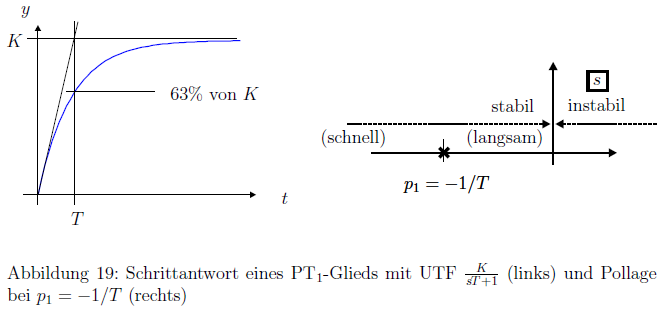
\includegraphics[width=15cm]{./images/PoleNullstellen.png}
		\end{center}
um eine schnelle Reaktion der Strecke
zu erreichen, sind grosse Werte am Reglerausgang nötig. Das bedeutet, dass man
T nicht beliebig klein machen kann, bzw. den Pol $p_1$ nicht beliebig weit nach links
legen darf.\\

Das $PT_2$-Glied hat eine UTF mit den drei Parametern K, $\xi$ und T (bzw. $\omega$ n = 1/T ).
\begin{equation}
\boxed{\frac{Y(s)}{R(s)}=G(s)=\frac{K}{s^2T^2+2\xi Ts+1}=\frac{K\omega^{2}_{n}}{s^2 + 2\xi \omega_{n}s+\omega^{2}_{n}}}
\end{equation}
\begin{itemize}
\item Modifikation
von K verändert die Höhe der Schrittantwort durch Strecken/Stauchen in
vertikaler Richtung. (Signalwerte)
\item Modifikation von T (bzw. $\omega n$) verändert
die Schrittantwort durch Strecken/Stauchen in horizontaler Richtung. (Zeit)
\item Abhängig von $\xi$ ergeben sich folgende Fälle:
\begin{itemize}
\item Fall mit $\xi$ < 0
Da T als positiv angenommen wird, ergibt sich für $\xi$ < 0 gemäss Vorzeichenbedingung
ein instabiles System.
\item Fall mit $\xi$ = 0
Dies ergibt einen harmonischen Oszillator; die Pole liegen bei $\pm j\omega_{n}$.
NB: die Periode der Oszillation entspricht nicht der Zeitkonstanten T.
\item Fall mit $ 0 < \xi < 1$
Hier resultiert ebenfalls eine Schwingung mit einer Periode; allerdings ist
die Schwingung gedämpft. Dieser Fall wird unten genauer betrachtet.
\item Fall mit $1 \leq \xi$
Dies entspricht dem aperiodischen Fall. Für (35) ist eine Faktorisierung
mit reellen Werten T1,2 möglich:
Für $\xi$ = 1 ist T1 = T2 = T; das $PT_2$-Glied entspricht der Serieschaltung
zweier identischer PT1-Glieder.
Für $\xi$ > 1 ist $T_1 > T > T_2$; das $PT_2$-Glied entspricht der Serieschaltung
zweier unterschiedlicher PT1-Glieder.
Für $\xi \gg 0$ wird mit $T_1 \gg T_2$ die Zeitkonstante T1 dominant. Das $PT_2$-
Glied verhält sich ähnlich wie ein $PT_1$-Glied
\end{itemize}
\end{itemize}

\[p_{1,2}=\frac{-2\xi\omega_n \pm \sqrt{4\xi^2 \omega^2_n - 4\omega^2_n}}{2}=\underbrace{-\xi\omega_n} \pm \underbrace{\sqrt{\xi^2-1}\cdot \omega_n}\]
\textcolor{white}{x} \hspace{10.5cm} $\sigma$ 
\hspace{1.5cm} $j\omega$
\begin{eqnarray}
\sigma=-\xi\omega_n \quad und \quad \omega=\sqrt{1-\xi^2}\cdot \omega_n  \quad bzw. \\ \omega_n=\sqrt{\omega^2 + \sigma^2}  \quad und  \quad \xi = -\frac{\sigma}{\omega_n}=-\frac{\sigma}{\sqrt{\omega^2 + \sigma^2}}\label{xiOmega}
\end{eqnarray}

Die Schrittantwort eines $PT_2$-Glieds mit $|\xi| < 1$ ergibt
\begin{equation}
\boxed{Y(s)=\frac{K\omega^2_n}{s(s^2+2\xi\omega_n s +\omega^2_n)}\laplace K\mathop{\Big[}1-e^{\sigma t}\mathop{\Big[}cos(\omega t)-\frac{\sigma}{\omega}sin(\omega t)\mathop{\Big]}\mathop{\Big]}=y(t)}
\end{equation}
\begin{multicols}{2}
\begin{itemize}
\item K ergibt sich durch $y_\infty$.
\item $\omega$ ergibt sich durch die Periode $T_\omega$ = 2$\pi$/$\omega$ [= $2T_m$].
\item $\sigma$ ergibt sich durch die Überschwingweite ym aus der Formel $y_m/y_\infty = e^{
\frac{\sigma}{\omega}\pi}$.
\item $\omega$n und $\xi$ ergeben sich gemäss (\ref{xiOmega}) aus $\omega$ und $\sigma$.
\end{itemize}
	\columnbreak
\begin{center}
	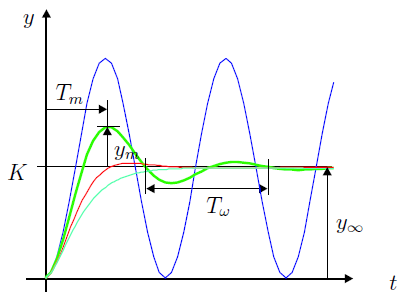
\includegraphics[width=6cm]{./images/pt2.png}
\end{center}
\end{multicols}

\subsubsection{Minimalphasigkeit}
Gegenüber den Polen werden die Nullstellen oft etwas vernachlässigt. Trotzdem
gibt es auch Fälle, in denen durch ungünstige Lage von Nullstellen regelungstechnische
Probleme erschwert werden. Beispiele sind Nullstellen in der rechten Halbebene,
durch die ein System nichtminimalphasig wird.
\subsubsection{Totzeit, Padé-Approximation}
\begin{equation}
\boxed{e^{-sT_t}=e^x\mathop\mid\limits{_{x=-sT_t}} \quad mit \quad e^x\approx 1 \approx \frac{2+x}{2-x} \approx \frac{12+6x+x^2}{12-6x+x^2} \approx \ldots}
\end{equation}
\begin{itemize}
\item  Sie ist stabil, unabhängig von der Ordnung.
\item  Die Nullstellen der Approximation entsprechen — an der Imaginärachse der
komplexen Ebene gespiegelt — den Polen. Beim Ersetzen eines Totzeitglieds
bleibt damit die Allpasseigenschaft erhalten mit $|G(j\omega)| = 1$. Weiter bleibt
auch die Nichtminimalphasigkeit erhalten.
\item  Ihr Phasengang konvergiert mit zunehmender Ordnung gegen denjenigen des
Totzeitglieds $e^{-sT_t} : \angle e^{-j\omega T_t} = -\omega T_t$.
\end{itemize}

\subsection{Blockdiagramm Algebra}
\begin{center}
	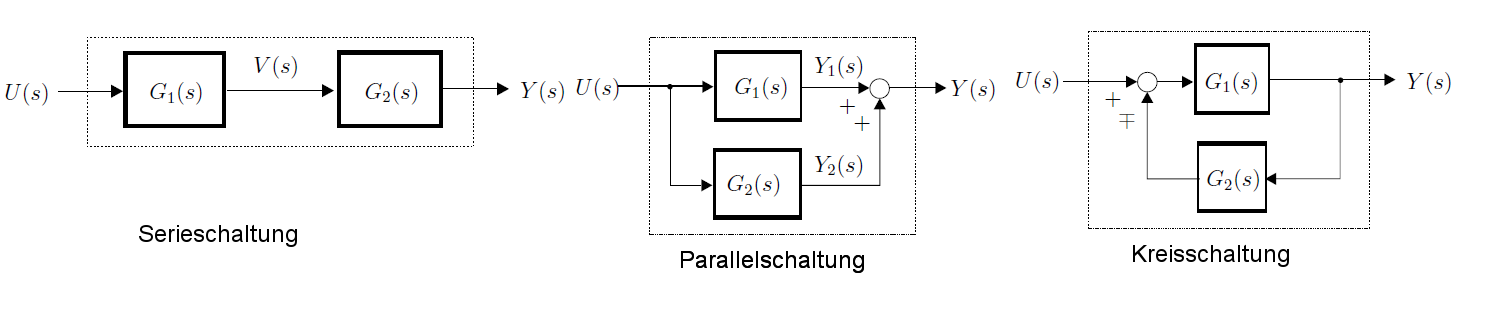
\includegraphics[width=16cm]{./images/blockdiagrammAlgebra.png}
\end{center}
\begin{itemize}
\item Zwei Blöcke hintereinander 
\begin{itemize}
	\item $U(s) \longrightarrow G_1(s)\longrightarrow G_2(s) \longrightarrow Y(s) \quad ergibt  \quad G(s)=G_1(s)\cdot G_2(s)$
	\item $Y(s) = G(s)=G_1(s)\cdot G_2(s) \cdot U(s)$
\end{itemize}
\item Zwei Blöcke Parallel
\begin{itemize}
	\item $G(s) = G_1(s) + G_2(s)$
	\item $Y_1(s) = G_1(s)\cdot U(s), Y_2(s) = G_2(s)\cdot U(s) \quad und \quad  Y(s) = Y_1(s)+ Y_2(s)$
	\item ergibt: $Y(s)= (G_s(s)+G_2(s))\cdot U(s)$
\end{itemize}

\item Kreisschaltung
\begin{itemize}
	\item $G(s) = \frac{G_1(s)}{1\pm G_1(s)\cdot G_2(s)}$
	\item $Y(s) = \frac{G_1(s)}{1\pm G_1(s)\cdot G_2(s)} \cdot U(s)$
\end{itemize}
\end{itemize}
\begin{center}
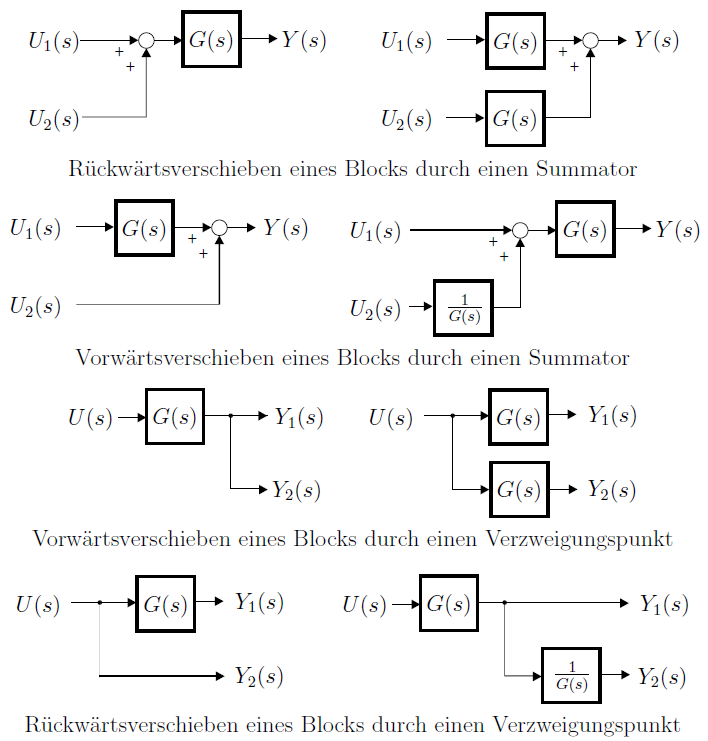
\includegraphics[width=8cm]{./images/blockdiagrammAlgebra2.png}
\end{center}


\subsection{Bodediagramm und Nyquistdiagramm}

\subsection{Stabilität allgemeines Nyquistkriterium}


\newpage